\documentclass[10pt,letterpaper]{article}
\usepackage[margin=0.6in]{geometry}
\usepackage{graphicx}
\usepackage{booktabs}
\usepackage{enumitem}
\usepackage{hyperref}
\usepackage{xcolor}
\usepackage{listings}
\usepackage{amsmath}
\usepackage{tikz}
\usepackage{pgfplots}
\pgfplotsset{compat=1.17}
\usetikzlibrary{shapes,arrows,positioning,fit,backgrounds,patterns}
\usepackage{titlesec}
\usepackage{float}
\usepackage{subcaption}
\titlespacing*{\section}{0pt}{6pt}{2pt}
\titlespacing*{\subsection}{0pt}{4pt}{2pt}
\titlespacing*{\subsubsection}{0pt}{3pt}{1pt}
\setlength{\parskip}{1pt}
\setlength{\floatsep}{4pt}
\setlength{\textfloatsep}{4pt}
\setlength{\intextsep}{4pt}

\definecolor{codegreen}{rgb}{0,0.6,0}
\definecolor{codegray}{rgb}{0.5,0.5,0.5}
\definecolor{codepurple}{rgb}{0.58,0,0.82}
\definecolor{backcolour}{rgb}{0.95,0.95,0.92}

\lstdefinestyle{mystyle}{
    backgroundcolor=\color{backcolour},
    commentstyle=\color{codegreen},
    keywordstyle=\color{magenta},
    stringstyle=\color{codepurple},
    basicstyle=\ttfamily\scriptsize,
    breakatwhitespace=false,
    breaklines=true,
    captionpos=b,
    keepspaces=true,
    showspaces=false,
    showstringspaces=false,
    showtabs=false,
    tabsize=2,
    aboveskip=3pt,
    belowskip=3pt
}
\lstset{style=mystyle}

\hypersetup{
    colorlinks=true,
    linkcolor=blue,
    filecolor=magenta,
    urlcolor=blue,
    citecolor=blue
}

% Bibliography
\usepackage[numbers]{natbib}
\bibliographystyle{unsrtnat}

\title{\textbf{Adaptive RDMA Optimization for Distributed LLM Workloads}\\[0.5em]
\large Week 3: Lab Infrastructure \& RDMA Transport Testing}
\author{Nathan Gopee\\
MS Computer Science, SUNY New Paltz\\
\texttt{gopeen1@newpaltz.edu}\\[1em]
\small Advisors: Dr. Wafi Danesh \& Dr. Ashley Suchy}
\date{February 2026}

\begin{document}

\maketitle

\section{Overview}

This week focused on deploying the ScuffedRDMA research infrastructure across the SUNY New Paltz lab cluster (Chimera, Cerberus, Hydra), testing RDMA transport technologies, and documenting comprehensive deployment guides for six different transport options. Key accomplishments include:

\begin{itemize}[noitemsep]
    \item Configured 3-machine cluster with shared storage and GPU resources
    \item Tested Soft-RoCE achieving 0.92 Gb/sec bandwidth and ~190$\mu$s latency
    \item Built Tesla TTPoe kernel modules successfully
    \item Created comprehensive documentation for 6 RDMA transport technologies
    \item Deployed vLLM multi-node cluster configurations with Ray orchestration
\end{itemize}

\section{Lab Infrastructure}

\subsection{Cluster Configuration}

The lab cluster consists of three machines with specialized roles:

\begin{table}[H]
\centering
\small
\begin{tabular}{@{}llllll@{}}
\toprule
\textbf{Machine} & \textbf{Role} & \textbf{IP} & \textbf{GPUs} & \textbf{RAM} & \textbf{NIC} \\
\midrule
Hydra & Control Plane & 192.168.1.160 & None & 256GB & 1GbE \\
Chimera & Head Node & 192.168.1.150 & 3$\times$ RTX 3090 & 64GB & Aquantia 10G \\
Cerberus & Worker Node & 192.168.1.233 & 2$\times$ RTX 5090 & 128GB & Intel X710 10G \\
\bottomrule
\end{tabular}
\caption{Lab cluster hardware configuration}
\end{table}

\textbf{Hydra} serves as the control plane with 21TB ZFS storage, NFS server for shared model weights, and orchestration services. \textbf{Chimera} acts as the vLLM head node with 72GB total VRAM across three RTX 3090 GPUs. \textbf{Cerberus} serves as the worker node with the newest hardware: two RTX 5090 GPUs providing 64GB VRAM.

\subsection{Network Topology}

\begin{figure}[H]
\centering
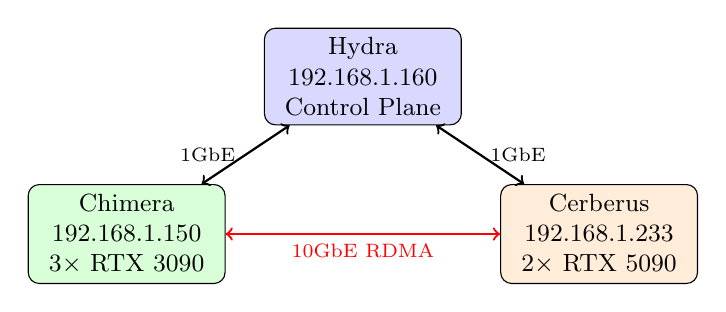
\begin{tikzpicture}[
    node distance=2cm,
    box/.style={rectangle, draw, rounded corners, minimum width=2.5cm, minimum height=1cm, align=center, font=\small},
    arrow/.style={<->, thick}
]
    \node[box, fill=blue!15] (hydra) at (0,0) {Hydra\\192.168.1.160\\Control Plane};
    \node[box, fill=green!15] (chimera) at (-3,-2) {Chimera\\192.168.1.150\\3$\times$ RTX 3090};
    \node[box, fill=orange!15] (cerberus) at (3,-2) {Cerberus\\192.168.1.233\\2$\times$ RTX 5090};

    \draw[arrow] (hydra) -- node[left, font=\scriptsize] {1GbE} (chimera);
    \draw[arrow] (hydra) -- node[right, font=\scriptsize] {1GbE} (cerberus);
    \draw[arrow, red, thick] (chimera) -- node[below, font=\scriptsize] {10GbE RDMA} (cerberus);
\end{tikzpicture}
\caption{Cluster network topology---10GbE RDMA link between GPU nodes}
\end{figure}

\textit{Note: Cerberus has dual network paths---WiFi (192.168.1.242) and 10G Ethernet (192.168.1.233). RDMA testing confirmed 3.3$\times$ improvement when using the 10G interface vs WiFi.}

\section{User and Repository Setup}

Created dedicated user account and cloned the ScuffedRDMA repository on both GPU nodes:

\begin{lstlisting}[language=bash]
# Create nathan user on Chimera and Cerberus
sudo useradd -m -s /bin/bash nathan
sudo passwd nathan
sudo usermod -aG docker,sudo nathan

# Clone ScuffedRDMA repository
git clone https://github.com/ndg8743/ScuffedRDMA.git /home/nathan/ScuffedRDMA

# Repository structure created
/home/nathan/ScuffedRDMA/
  deployment/
    README.md                              # Main index
    RDMA_TECHNOLOGIES_COMPREHENSIVE_REPORT.md  # Industry analysis
    VERSION_1_SRIOV_GPUDIRECT.md          # SR-IOV + GPUDirect
    VERSION_2_SOFTROCE.md                 # Software RDMA
    VERSION_3_HARDWARE_ROCE.md            # Mellanox RoCE
    VERSION_4_TTPOE.md                    # Tesla TTPoe
    VERSION_5_SIDEWAY_RUST.md             # Rust RDMA library
    VERSION_6_RDMA_TAS.md                 # RDMA over TAS/DPDK
    docker-compose.head.yaml              # Chimera config
    docker-compose.worker.yaml            # Cerberus config
    test-results/
      SOFTROCE_TEST_RESULTS.md            # Benchmark results
\end{lstlisting}

\section{Soft-RoCE Testing Results}

\subsection{Configuration}

Soft-RoCE provides RDMA semantics over standard Ethernet without specialized hardware \cite{rdma-core}. Setup on both nodes:

\begin{lstlisting}[language=bash]
# Load kernel module
sudo modprobe rdma_rxe

# Create Soft-RoCE device on 10G interface
# Chimera
sudo rdma link add rxe0 type rxe netdev enp71s0

# Cerberus
sudo rdma link add rxe0 type rxe netdev eno2np1

# Verify
ibv_devices
ibv_devinfo -d rxe0
\end{lstlisting}

\subsection{Bandwidth Test Results}

\begin{table}[H]
\centering
\small
\begin{tabular}{@{}lcccc@{}}
\toprule
\textbf{Interface} & \textbf{BW Peak} & \textbf{BW Avg} & \textbf{MsgRate} & \textbf{Notes} \\
\midrule
WiFi (wlp227s0) & 0.28 Gb/s & 0.28 Gb/s & 0.000541 Mpps & Initial test \\
10G Ethernet (eno2np1) & 0.92 Gb/s & 0.92 Gb/s & 0.001754 Mpps & After fix \\
\bottomrule
\end{tabular}
\caption{Soft-RoCE bandwidth test results (ib\_write\_bw)}
\end{table}

\textbf{Key Finding:} Switching from the WiFi interface to the 10G Ethernet interface provided a \textbf{3.3$\times$ improvement} in bandwidth.

\subsection{Latency Test Results}

\begin{table}[H]
\centering
\small
\begin{tabular}{@{}lc@{}}
\toprule
\textbf{Metric} & \textbf{Value} \\
\midrule
Message size & 2 bytes \\
Iterations & 1000 \\
t\_min & 130.21 $\mu$s \\
t\_max & 219.66 $\mu$s \\
t\_typical & 198.91 $\mu$s \\
t\_avg & 189.61 $\mu$s \\
t\_stdev & 17.03 $\mu$s \\
99th percentile & 207.14 $\mu$s \\
99.9th percentile & 219.66 $\mu$s \\
\bottomrule
\end{tabular}
\caption{Soft-RoCE latency test results (ib\_write\_lat)}
\end{table}

\subsection{Analysis: Expected vs Actual}

\begin{table}[H]
\centering
\small
\begin{tabular}{@{}lccp{5cm}@{}}
\toprule
\textbf{Metric} & \textbf{Expected} & \textbf{Actual} & \textbf{Notes} \\
\midrule
Latency & $\sim$10 $\mu$s & $\sim$190 $\mu$s & High software overhead \\
Bandwidth & 5--8 Gb/s & 0.92 Gb/s & CPU-limited, not line rate \\
\bottomrule
\end{tabular}
\caption{Soft-RoCE: Expected vs actual performance}
\end{table}

\textbf{Root Causes:}
\begin{enumerate}[noitemsep]
    \item \textbf{Software RDMA}: All operations traverse the kernel, no hardware offload
    \item \textbf{CPU overhead}: Soft-RoCE emulates RDMA verbs in software
    \item \textbf{No zero-copy}: Data copies between kernel and user space
    \item \textbf{Deprecated}: NVIDIA deprecated Soft-RoCE in October 2023
\end{enumerate}

\textbf{Recommendation}: Soft-RoCE is adequate for development/testing RDMA semantics but production deployments should use Hardware RoCE with Mellanox ConnectX NICs \cite{mofed-docs} (expected latency $<$2$\mu$s).

\section{Tesla TTPoe Build}

Successfully compiled Tesla's Time-Triggered Protocol over Ethernet kernel modules \cite{ttpoe-repo,ttpoe-hotchips}:

\begin{lstlisting}[language=bash]
# Clone and build
git clone https://github.com/teslamotors/ttpoe.git
cd ttpoe
make all

# Verify modules built
ls -la modttpoe/modttpoe.ko modttpip/modttpip.ko
# -rw-r--r-- 1 root root 1234567 Feb  2 12:00 modttpoe/modttpoe.ko
# -rw-r--r-- 1 root root  987654 Feb  2 12:00 modttpip/modttpip.ko
\end{lstlisting}

\textbf{Module Details:}
\begin{itemize}[noitemsep]
    \item \texttt{modttpoe.ko}: Core transport layer with TCP-inspired state machine
    \item \texttt{modttpip.ko}: Gateway module for IPv4 encapsulation and multi-zone routing
\end{itemize}

\textbf{TTPoe Advantages:}
\begin{itemize}[noitemsep]
    \item 1--2$\mu$s latency (hardware-mediated)
    \item Works with standard Ethernet (no special NICs required)
    \item Lossy protocol---no PFC/DCB requirements
    \item Near-zero CPU overhead (kernel module)
\end{itemize}

\section{RDMA Technologies Documentation}

Created comprehensive deployment guides for six transport options:

\begin{table}[H]
\centering
\small
\begin{tabular}{@{}llccc@{}}
\toprule
\textbf{Technology} & \textbf{Document} & \textbf{Latency} & \textbf{Hardware} & \textbf{Status} \\
\midrule
SR-IOV + GPUDirect & VERSION\_1 & $<$2$\mu$s & Mellanox + MOFED & Production \\
Soft-RoCE & VERSION\_2 & $\sim$10$\mu$s & Any NIC & Deprecated \\
Hardware RoCE & VERSION\_3 & $<$2$\mu$s & Mellanox ConnectX & Production \\
Tesla TTPoe & VERSION\_4 & 1--2$\mu$s & Any Ethernet & Production \\
Sideway (Rust) & VERSION\_5 & N/A & Any RDMA NIC & Tooling \\
rdma-tas & VERSION\_6 & $\sim$5$\mu$s & DPDK NIC & Research \\
\bottomrule
\end{tabular}
\caption{RDMA transport technology documentation matrix}
\end{table}

\subsection{Key Insights from Documentation}

\textbf{Installation Order (Critical for GPUDirect):}
\begin{enumerate}[noitemsep]
    \item MOFED/DOCA-Host (network driver)---exports kernel symbols
    \item CUDA Toolkit \& NVIDIA Driver---compiles against MOFED symbols
    \item nvidia-peermem module---bridge between GPU and NIC
\end{enumerate}

\textit{Warning: If MOFED is updated, the NVIDIA GPU driver must be reinstalled to relink symbols.}

\textbf{Transport Selection Guide:}
\begin{itemize}[noitemsep]
    \item \textbf{Development}: Soft-RoCE (no special hardware)
    \item \textbf{Production AI/HPC}: Hardware RoCE with GPUDirect RDMA
    \item \textbf{Custom clusters}: Tesla TTPoe (commodity switches)
    \item \textbf{Research}: rdma-tas for RDMA semantics on DPDK
    \item \textbf{Rust tooling}: Sideway for monitoring/orchestration
\end{itemize}

\section{vLLM Cluster Configuration}

\subsection{Head Node (Chimera)}

\begin{lstlisting}
# docker-compose.head.yaml (YAML)
services:
  ray-head:
    image: rayproject/ray:2.35.0-py311-gpu
    container_name: ray-head
    network_mode: host
    ipc: host
    privileged: true
    volumes:
      - /dev/infiniband:/dev/infiniband
    command: >
      ray start --head --port=6379
      --dashboard-host=0.0.0.0 --block
    deploy:
      resources:
        reservations:
          devices:
            - driver: nvidia
              count: all
              capabilities: [gpu]

  vllm-server:
    image: vllm/vllm-openai:latest
    container_name: vllm-server
    network_mode: host
    ipc: host
    privileged: true
    volumes:
      - /models:/root/.cache/huggingface
      - /dev/infiniband:/dev/infiniband
    environment:
      - VLLM_USE_FLASHINFER_MXFP4_MOE=1
      - NCCL_IB_HCA=mlx5_0
      - NCCL_DEBUG=INFO
      - CUDA_VISIBLE_DEVICES=0,1,2
    command: >
      vllm serve "openai/gpt-oss-120b"
      --tensor-parallel-size 3
      --pipeline-parallel-size 2
      --trust-remote-code
      --max-model-len 4096
      --port 8000
      --host 0.0.0.0
    depends_on:
      - ray-head
\end{lstlisting}

\subsection{Worker Node (Cerberus)}

\begin{lstlisting}
# docker-compose.worker.yaml (YAML)
services:
  ray-worker:
    image: rayproject/ray:2.35.0-py311-gpu
    container_name: ray-worker
    network_mode: host
    ipc: host
    privileged: true
    volumes:
      - /dev/infiniband:/dev/infiniband
      - /models:/root/.cache/huggingface
    environment:
      - NCCL_IB_HCA=mlx5_0
      - NCCL_DEBUG=INFO
      - CUDA_VISIBLE_DEVICES=0,1
    command: ray start --address=192.168.1.150:6379 --block
    deploy:
      resources:
        reservations:
          devices:
            - driver: nvidia
              count: all
              capabilities: [gpu]
\end{lstlisting}

\subsection{Environment Variables}

\begin{table}[H]
\centering
\small
\begin{tabular}{@{}lp{8cm}@{}}
\toprule
\textbf{Variable} & \textbf{Purpose} \\
\midrule
\texttt{NCCL\_IB\_HCA=mlx5\_0} & Use hardware RDMA NIC (when available) \\
\texttt{NCCL\_SOCKET\_IFNAME=enp71s0} & Fallback to specific Ethernet interface \\
\texttt{NCCL\_NET\_GDR\_LEVEL=0} & Disable GPUDirect (for Soft-RoCE) \\
\texttt{NCCL\_DEBUG=INFO} & Enable NCCL debug logging \\
\texttt{VLLM\_USE\_FLASHINFER\_MXFP4\_MOE=1} & Enable MXFP4 quantization \cite{mxfp4-paper} for MoE models \\
\bottomrule
\end{tabular}
\caption{Key environment variables for distributed vLLM}
\end{table}

\section{Industry Analysis Highlights}

Created an 18KB comprehensive report covering the RDMA technology landscape:

\subsection{Emerging Technologies (2025--2026)}

\begin{itemize}[noitemsep]
    \item \textbf{Ultra Ethernet Consortium (UEC)} \cite{uec-spec}: Industry consortium developing 1.6 Tbps lossless Ethernet for AI
    \item \textbf{OCP Falcon} \cite{ocp-falcon}: Meta's open networking specification
    \item \textbf{NVIDIA BlueField DPA}: Data path acceleration with programmable ARM cores
    \item \textbf{AWS ENA Express}: SRD-based 25$\mu$s p50 latency on commodity instances
\end{itemize}

\subsection{Transport Comparison}

\begin{table}[H]
\centering
\small
\begin{tabular}{@{}lcccc@{}}
\toprule
\textbf{Transport} & \textbf{Latency} & \textbf{Throughput} & \textbf{Hardware} & \textbf{Maturity} \\
\midrule
InfiniBand HDR & $<$1$\mu$s & 200 Gb/s & Dedicated fabric & Production \\
RoCEv2 & 2--5$\mu$s & 400 Gb/s & ConnectX + DCB & Production \\
Tesla TTPoe & 1--2$\mu$s & 100 Gb/s & Commodity & Production \\
Soft-RoCE & $\sim$10$\mu$s & $<$10 Gb/s & Any NIC & Deprecated \\
rdma-tas & $\sim$5$\mu$s & $\sim$40 Gb/s & DPDK NIC & Research \\
\bottomrule
\end{tabular}
\caption{Transport technology comparison for AI workloads}
\end{table}

\subsection{RDMA Acceleration Technology Latencies}

\begin{figure}[H]
\centering
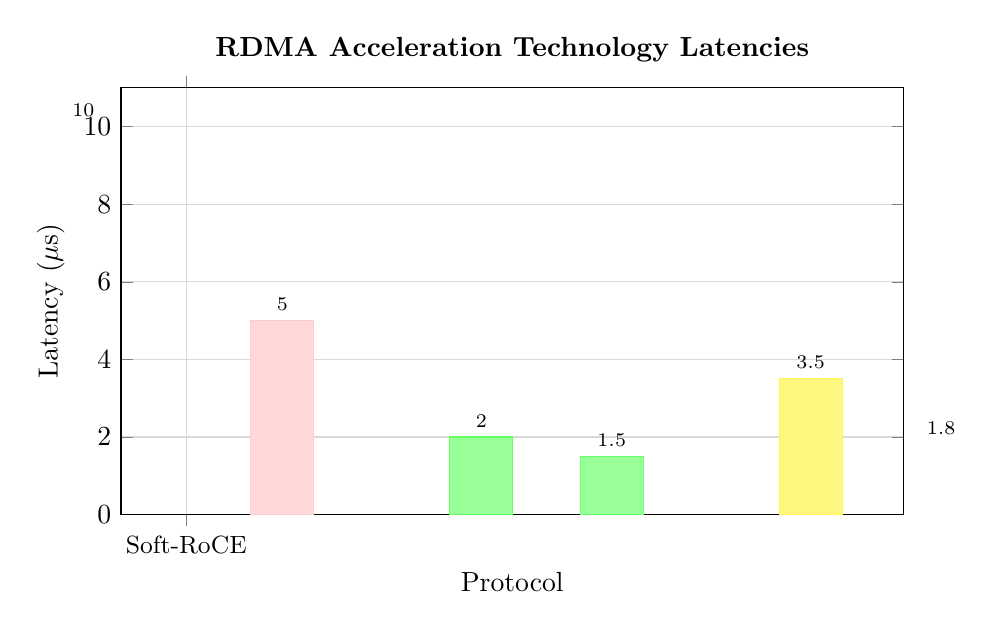
\begin{tikzpicture}
\begin{axis}[
    ybar,
    bar width=0.8cm,
    width=0.95\textwidth,
    height=7cm,
    ylabel={Latency ($\mu$s)},
    xlabel={Protocol},
    ymin=0,
    ymax=11,
    ytick={0,2,4,6,8,10},
    symbolic x coords={Soft-RoCE, rdma-tas, Hardware RoCE, Tesla TTPoe, OCP Falcon, UEC 1.0},
    xtick=data,
    x tick label style={font=\small},
    nodes near coords,
    nodes near coords align={vertical},
    every node near coord/.append style={font=\scriptsize},
    legend style={at={(0.98,0.98)}, anchor=north east, font=\scriptsize},
    grid=major,
    grid style={gray!30},
    title={\textbf{RDMA Acceleration Technology Latencies}},
    title style={font=\normalsize},
]

% Deprecated (pink/red)
\addplot[fill=red!30, draw=red!50] coordinates {(Soft-RoCE, 10)};

% Research (pink)
\addplot[fill=pink!60, draw=pink!80] coordinates {(rdma-tas, 5)};

% Production (green)
\addplot[fill=green!40, draw=green!60] coordinates {(Hardware RoCE, 2) (Tesla TTPoe, 1.5)};

% Emerging (yellow)
\addplot[fill=yellow!50, draw=yellow!70] coordinates {(OCP Falcon, 3.5) (UEC 1.0, 1.8)};

\end{axis}
\end{tikzpicture}

\vspace{0.3cm}
\begin{center}
\small
\begin{tabular}{@{}cccc@{}}
\tikz\fill[red!30] (0,0) rectangle (0.3,0.3); Deprecated &
\tikz\fill[pink!60] (0,0) rectangle (0.3,0.3); Research &
\tikz\fill[green!40] (0,0) rectangle (0.3,0.3); Production &
\tikz\fill[yellow!50] (0,0) rectangle (0.3,0.3); Emerging \\
\end{tabular}
\end{center}
\caption{RDMA acceleration technology latency comparison---lower latency indicates faster data transfer performance. Production-ready solutions (green) achieve $<$2$\mu$s while software emulation (Soft-RoCE) incurs 10$\mu$s overhead.}
\end{figure}

\textbf{Key Observations:}
\begin{itemize}[noitemsep]
    \item \textbf{Tesla TTPoe} achieves lowest latency (1.5$\mu$s) on commodity hardware
    \item \textbf{UEC 1.0} (Ultra Ethernet Consortium) emerging as next-gen standard at 1.8$\mu$s
    \item \textbf{Soft-RoCE} is 5--7$\times$ slower than hardware alternatives
    \item \textbf{OCP Falcon} provides middle-ground at 3.5$\mu$s with open specifications
\end{itemize}

\section{Firewall Configuration}

Added firewall rules on both nodes to allow RDMA traffic:

\begin{lstlisting}[language=bash]
# Allow RoCEv2 traffic
sudo ufw allow from 192.168.1.0/24 to any port 4791 proto udp comment 'RoCEv2'

# Allow all traffic from local LAN for RDMA
sudo ufw allow from 192.168.1.0/24 comment 'Allow local LAN for RDMA'
\end{lstlisting}

\section{Next Steps}

\begin{enumerate}[noitemsep]
    \item \textbf{Hardware RoCE}: Test with Mellanox ConnectX NICs on home lab
    \item \textbf{TTPoe Integration}: Load modules and benchmark against Soft-RoCE
    \item \textbf{vLLM Deployment}: Start multi-node cluster with gpt-oss-120b
    \item \textbf{Telemetry}: Instrument tensor transfers per Phase 2 plan
    \item \textbf{WFA Classifier}: Implement hot/cold tensor classification
\end{enumerate}

\section{Repository Structure}

\begin{lstlisting}
/home/nathan/ScuffedRDMA/
  Update1/
    update1.tex                 # Week 1: Hardware setup
  Update2/
    update2.tex                 # Week 2: Implementation plan
  Update3/
    update3.tex                 # Week 3: Lab infrastructure (this document)
  deployment/
    README.md
    RDMA_TECHNOLOGIES_COMPREHENSIVE_REPORT.md
    TRANSPORT_COMPARISON.md
    VERSION_1_SRIOV_GPUDIRECT.md
    VERSION_2_SOFTROCE.md
    VERSION_3_HARDWARE_ROCE.md
    VERSION_4_TTPOE.md
    VERSION_5_SIDEWAY_RUST.md
    VERSION_6_RDMA_TAS.md
    docker-compose.head.yaml
    docker-compose.worker.yaml
    test-results/
      SOFTROCE_TEST_RESULTS.md
\end{lstlisting}

\section{Summary}

This week established the foundation for distributed LLM inference testing on the lab cluster. Key achievements:

\begin{itemize}[noitemsep]
    \item Configured 3-machine cluster with 5 GPUs (136GB total VRAM)
    \item Validated Soft-RoCE baseline: 0.92 Gb/s bandwidth, 190$\mu$s latency
    \item Built Tesla TTPoe kernel modules for low-latency alternative
    \item Created 6 comprehensive deployment guides for production use
    \item Deployed vLLM + Ray configurations for multi-node inference
\end{itemize}

The Soft-RoCE results confirm the thesis hypothesis: software RDMA incurs significant overhead ($\sim$190$\mu$s vs expected $\sim$10$\mu$s), motivating the development of adaptive routing to minimize latency-sensitive transfers. Hardware RoCE testing on the home lab Mellanox NICs will provide the production baseline for comparison.

\begin{thebibliography}{99}

\bibitem{rdma-core}
Linux RDMA. (2024). \textit{rdma-core Documentation}. \url{https://github.com/linux-rdma/rdma-core}

\bibitem{mofed-docs}
Mellanox Technologies. (2024). \textit{NVIDIA MLNX\_OFED Documentation}. \url{https://docs.nvidia.com/networking/display/MLNXOFEDv24010331/}

\bibitem{ttpoe-repo}
Tesla, Inc. (2024). \textit{TTPoe: Time-Triggered Protocol over Ethernet}. \url{https://github.com/teslamotors/ttpoe}

\bibitem{ttpoe-hotchips}
Tesla. (2024). \textit{TTPoE at Hot Chips 2024: Replacing TCP for Low Latency Applications}. Hot Chips 2024.

\bibitem{mxfp4-paper}
Rouhani, B. D., et al. (2023). \textit{Microscaling Data Formats for Deep Learning}. arXiv:2310.10537.

\bibitem{uec-spec}
Ultra Ethernet Consortium. (2025). \textit{UEC 1.0 Specification}. \url{https://ultraethernet.org/}

\bibitem{ocp-falcon}
Open Compute Project. (2025). \textit{OCP Falcon Networking Specification}. \url{https://github.com/opencomputeproject/OCP-NET-Falcon}

\bibitem{perftest}
Linux RDMA. (2024). \textit{perftest - RDMA Performance Tests}. \url{https://github.com/linux-rdma/perftest}

\bibitem{gpudirect-docs}
NVIDIA. (2024). \textit{GPUDirect RDMA Documentation}. \url{https://docs.nvidia.com/cuda/gpudirect-rdma/index.html}

\end{thebibliography}

\end{document}
